% =====================================================================
\chapter{Risque et limites de l'arbitrage}
\label{ch:17}
% =====================================================================

\section{Objectifs et organisation du chapitre}

\paragraph{Objectifs.} Une stratégie d'arbitrage statistique gagne souvent un peu et perd rarement beaucoup. Le risque se concentre dans quelques épisodes : une paire qui se rompt, un écart qui s'élargit avant de converger, une foule d'arbitragistes qui liquident en même temps. À la fin du chapitre, vous saurez : (1) dimensionner une position avec le critère de Kelly et comprendre pourquoi on n'en utilise qu'une fraction ; (2) choisir et calibrer des protections contre la rupture d'une paire ; (3) expliquer, chiffres à l'appui, pourquoi un arbitrage \og certain\fg{} peut ruiner celui qui le porte ; (4) mesurer ce que vaut réellement la diversification entre paires ; (5) recenser les risques non statistiques (plateforme, contrepartie, réglementation, règles des \emph{prop firms}) et fixer des limites de risque.

\paragraph{Code.}\sloppy \texttt{code/ch17/ch17\_risk.py} (expériences E1 à E4) ; module \texttt{src/arbhub/risk/sizing.py} et ses tests \texttt{tests/test\_risk.py}.

% =====================================================================
\section{Combien miser ? Le critère de Kelly}
% =====================================================================

\subsection{Croissance logarithmique}

On investit à chaque période une fraction $f$ de sa richesse (le \emph{levier}) dans une stratégie de rendement $r_t$, d'espérance $\mu$ et de variance $\sigma^2$ par période. La richesse évolue selon $W_{t+1} = W_t(1 + f r_t)$, donc après $T$ périodes
\[
\ln W_T = \ln W_0 + \sum_{t=1}^{T}\ln(1 + f r_t).
\]
Par la loi des grands nombres, le taux de croissance $\frac1T\ln(W_T/W_0)$ converge vers $g(f) = \E[\ln(1+fr)]$. Le critère de Kelly \citep{kelly1956} choisit $f$ pour maximiser ce taux.

\begin{proposition}[Kelly en temps continu, \citet{thorp2006}]\label{c17:prop:kelly}
Pour des rendements petits, $g(f) \approx f\mu - \tfrac12 f^2\sigma^2$, maximal en
\[
f^\star = \frac{\mu}{\sigma^2}, \qquad g(f^\star) = \frac{\mu^2}{2\sigma^2} = \frac{SR^2}{2},
\]
où $SR = \mu/\sigma$ est le Sharpe par période. De plus $g(2f^\star) = 0$ : avec le double du levier de Kelly, la richesse ne croît plus.
\end{proposition}
\begin{proof}
Le développement $\ln(1+u) = u - u^2/2 + O(u^3)$ appliqué à $u = fr$ donne $\E[\ln(1+fr)] \approx f\E[r] - \tfrac12 f^2\E[r^2]$. Pour des rendements par période petits, $\E[r^2] = \sigma^2 + \mu^2 \approx \sigma^2$. La fonction $g(f) = f\mu - \tfrac12 f^2\sigma^2$ est une parabole tournée vers le bas ; sa dérivée $\mu - f\sigma^2$ s'annule en $f^\star = \mu/\sigma^2$, et $g(f^\star) = \mu^2/\sigma^2 - \tfrac12\mu^2/\sigma^2 = \mu^2/(2\sigma^2)$. Enfin $g(2f^\star) = 2\mu^2/\sigma^2 - \tfrac12\cdot4\mu^2/\sigma^2 = 0$.
\end{proof}

\begin{intuition}
La croissance est une colline. Jusqu'au sommet ($f^\star$), plus de levier fait monter plus vite. Après le sommet, chaque unité de levier supplémentaire ajoute plus de volatilité qu'elle n'ajoute de rendement, et la volatilité \emph{détruit} la croissance : perdre 50\,\% puis gagner 50\,\% laisse 75\,\% du capital. À deux fois le sommet, on est revenu au niveau de la mer : en moyenne arithmétique on gagne, en médiane on stagne.
\end{intuition}

\subsection{Kelly en pratique}

\begin{codebox}[ — E1, stratégie de Sharpe annuel 1 (rendement 10\,\%, volatilité 10\,\% sans levier), 4\,000 trajectoires de 10 ans]
Le levier de Kelly vaut $f^\star = 0{,}10/0{,}10^2 = 10$, soit une volatilité de 100\,\% par an.
\begin{center}\small
\setlength{\tabcolsep}{4pt}
\begin{tabular}{rrcccc}
\toprule
Fraction & Levier & Croissance & P(perte & P(drawdown & Drawdown \\
de Kelly & & médiane & à 10 ans) & $>50\,\%$) & médian \\
\midrule
0,10 & 1 & 10,0\,\%/an & 0,2\,\% & 0\,\% & 15,8\,\% \\
0,25 & 2,5 & 24,6\,\%/an & 0,3\,\% & 9,1\,\% & 36,1\,\% \\
0,50 & 5 & 45,9\,\%/an & 0,9\,\% & 86,5\,\% & 61,6\,\% \\
1,00 & 10 & 66,0\,\%/an & 5,4\,\% & 100\,\% & 89,6\,\% \\
1,50 & 15 & 46,5\,\%/an & 21,6\,\% & 100\,\% & 98,5\,\% \\
2,00 & 20 & $-0{,}8$\,\%/an & 50,4\,\% & 100\,\% & 99,9\,\% \\
\bottomrule
\end{tabular}
\end{center}
\textbf{Erreur d'estimation :} si l'on estime $f^\star$ sur 3 ans d'historique de cette même stratégie, l'estimation médiane est juste ($10{,}0$), mais 10\,\% des estimations sont sous $2{,}4$ et 10\,\% au-dessus de $17{,}5$ ; dans 4,2\,\% des cas on estime plus du double du vrai $f^\star$ (zone de croissance négative), et dans 4,7\,\% un $f^\star$ négatif.
\end{codebox}

\begin{figure}[h]
\centering
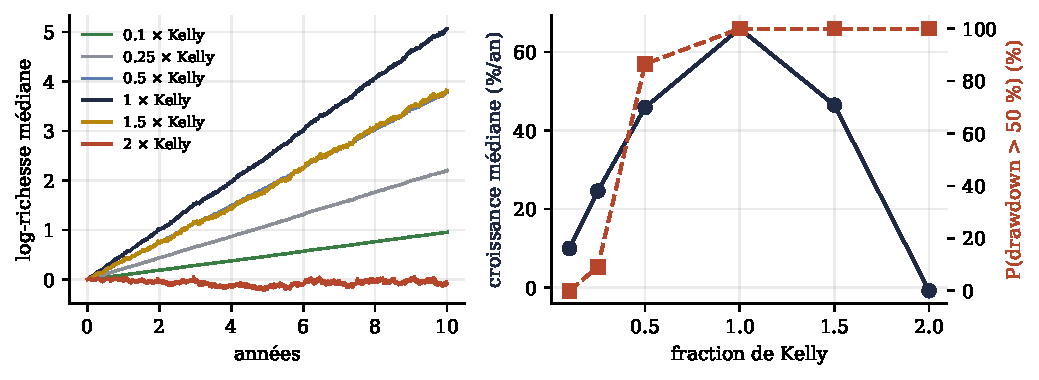
\includegraphics[width=0.95\textwidth]{ch17/kelly.pdf}
\caption{À gauche, log-richesse médiane selon la fraction de Kelly (les courbes à 0,5 et 1,5 Kelly se superposent : la croissance est symétrique autour du sommet). À droite, croissance médiane et probabilité de subir un drawdown de plus de 50\,\%.}
\label{c17:fig:kelly}
\end{figure}

\paragraph{Lecture.} Kelly maximise la croissance \emph{à long terme} en acceptant des drawdowns que presque personne ne supporte (90\,\% en médiane). La croissance est symétrique autour de $f^\star$ (0,5 et 1,5 Kelly croissent au même rythme), mais le risque ne l'est pas : la sur-estimation est bien plus coûteuse que la sous-estimation. Comme $f^\star$ est estimé avec une erreur énorme, la pratique professionnelle est d'utiliser entre un dixième et un quart de Kelly. Pour une stratégie de paires, rappelez-vous en outre que le Sharpe d'un \emph{backtest} est surestimé (chapitre~16) : le Kelly calculé sur un \emph{backtest} est doublement trop grand.

\subsection{Ciblage de volatilité}

Une alternative simple consiste à fixer une volatilité cible $\sigma^\ast$ (par exemple 10\,\% par an) et à dimensionner à chaque date
\[
w_t = \min\!\Big(\frac{\sigma^\ast}{\hat\sigma_t},\ L_{\max}\Big),
\]
où $\hat\sigma_t$ est la volatilité du P\&L par unité de position estimée sur une fenêtre passée, et $L_{\max}$ un levier plafond. C'est la fonction \texttt{vol\_target\_weights} du module ; son test vérifie qu'elle n'utilise que le passé et qu'elle atteint la cible sur des données stables. Le ciblage réduit la taille quand la volatilité monte, ce qui protège partiellement des épisodes de crise, mais avec un retard égal à la fenêtre d'estimation.

% =====================================================================
\section{Se protéger de la rupture d'une paire}
% =====================================================================

Le chapitre~1 a montré qu'une paire rompue transforme une règle de retour à la moyenne en machine à accumuler des pertes. On compare ici cinq protections.

\begin{description}
\item[Stop-loss en $z$.] On ferme si $|z_t| > z_{\text{stop}}$ (3 ou 4), et l'on ne rouvre que si $|z|$ redescend sous le seuil d'entrée.
\item[Stop-loss en durée.] On ferme si la position est ouverte depuis plus de trois demi-vies : un écart qui revient à la moyenne devrait s'être largement refermé dans ce délai (chapitre~5).
\item[Alarme CUSUM.] On surveille les innovations $e_t = s_t - \hat\varphi s_{t-1}$, qui doivent rester un bruit blanc de moyenne et d'écart-type connus si la relation est stable. Le CUSUM de \citet{page1954} cumule les écarts standardisés $z_t = (e_t - m)/d$ au-delà d'une marge $k$ :
\[
S^+_t = \max(0, S^+_{t-1} + z_t - k), \qquad S^-_t = \max(0, S^-_{t-1} - z_t - k),
\]
et déclenche une alarme dès que $S^+_t$ ou $S^-_t$ dépasse $h$. Une alarme retire la paire.
\item[$\hat\varphi$ glissant.] On suspend la paire tant que $\hat\varphi$ estimé sur les 120 derniers jours dépasse $0{,}98$.
\end{description}

\begin{intuition}
Le CUSUM est un compteur de \og petits mauvais signes\fg. Un jour légèrement anormal ne fait rien ($k$ absorbe le bruit), mais une série de jours anormaux dans le même sens s'accumule jusqu'à l'alarme. C'est la logique du contrôle qualité industriel, pour lequel il a été inventé : une machine déréglée produit des pièces un peu trop grandes, jour après jour.
\end{intuition}

\begin{codebox}[ — E2, cinq protections, 300 mondes par scénario]
\textbf{Protocole :} écart AR(1) avec $\varphi = 0{,}9$, formation de 500 jours, trading de 1\,000 jours, règle $|z|>2$, coûts 5 pb. Scénario \og rupture\fg{} : au 400\textsuperscript{e} jour de trading, l'écart devient une marche aléatoire avec une légère dérive. CUSUM avec $k = 0{,}5$ et $h = 10$. \textbf{Gain moyen (quantile 5\,\%) :}
\begin{center}\small
\begin{tabular}{lcc}
\toprule
Protection & Relation stable & Rupture \\
\midrule
Aucune & 63,7 (33,1) & $-22{,}2$ ($-70{,}5$) \\
Stop $|z| > 3$ & 58,7 (32,3) & 20,0 (0,3) \\
Stop $|z| > 4$ & 63,4 (33,1) & 20,0 ($-2{,}1$) \\
Stop en durée (3 demi-vies) & 54,6 (26,6) & 19,3 (0,0) \\
CUSUM & 60,8 (29,6) & 23,6 (4,9) \\
$\hat\varphi$ glissant & 63,7 (33,1) & $-4{,}1$ ($-37{,}0$) \\
\bottomrule
\end{tabular}
\end{center}
\textbf{CUSUM :} fausse alarme dans 7\,\% des mondes stables ; alarme après la rupture dans 96,7\,\% des mondes qui rompent, avec un délai médian de 53 jours.
\end{codebox}

\begin{figure}[h]
\centering
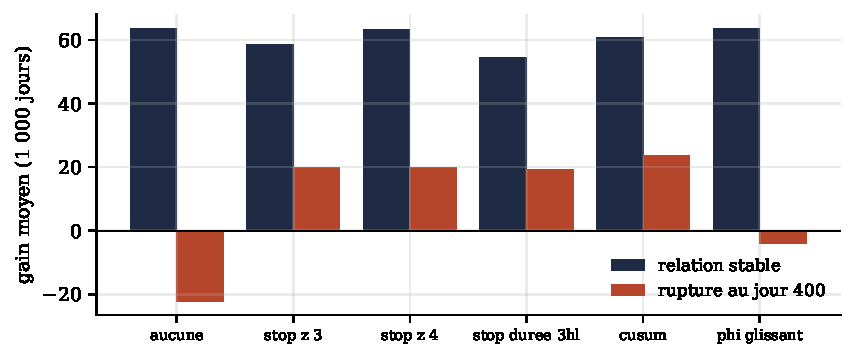
\includegraphics[width=0.8\textwidth]{ch17/protections_rupture.pdf}
\caption{Gain moyen selon la protection, avec une relation stable et avec une rupture au 400\textsuperscript{e} jour.}
\label{c17:fig:protect}
\end{figure}

\paragraph{Lecture.} (1) Le stop à $|z|>4$ est presque gratuit quand la relation est stable (63,4 contre 63,7) et transforme une perte moyenne de 22 en gain de 20 quand elle rompt : c'est la meilleure assurance par unité de coût. (2) Le stop à 3 coûte davantage (il coupe des écarts qui seraient revenus). (3) Le CUSUM offre la meilleure protection en cas de rupture et ne coûte que 3 en monde stable, au prix d'un calibrage (avec $k = 0{,}25$ et $h = 8$, un premier essai, il déclenchait à tort dans 94\,\% des mondes stables). (4) Le $\hat\varphi$ glissant ne déclenche jamais à tort mais réagit trop lentement : il faut 120 jours pour que l'estimation reflète le nouveau régime. Dans la pratique, on combine un stop en $z$ (protection immédiate) et un indicateur statistique (pour retirer durablement la paire).

\begin{pitfall}
Ces protections ont été évaluées dans un monde où l'on connaît la date de rupture. Dans la réalité, chaque déclenchement est ambigu : écart extrême mais temporaire, ou rupture ? Le stop vend souvent au pire moment, juste avant la convergence. Calibrer les seuils sur l'historique d'une paire est un nouveau choix de paramètres, à compter dans le nombre d'essais (chapitre~16).
\end{pitfall}

% =====================================================================
\section{Les limites de l'arbitrage}
% =====================================================================

\subsection{L'argument de Shleifer et Vishny}

\citet{shleifer1997} partent d'un constat : l'arbitrage est réalisé par peu d'acteurs spécialisés qui utilisent un capital emprunté (marge, levier) ou délégué (investisseurs d'un fonds). Quand un écart s'élargit avant de converger, l'arbitragiste subit des pertes latentes ; ses prêteurs exigent de la marge supplémentaire, ses investisseurs retirent leur argent, et il doit liquider \emph{au moment où l'opportunité est la meilleure}. Sa vente élargit encore l'écart. L'arbitrage est donc le plus contraint précisément quand il serait le plus utile. \citet{brunnermeier2009} formalisent cette spirale entre liquidité de financement et liquidité de marché ; \citet{mitchell2010} documentent des écarts d'arbitrage qui sont restés ouverts des mois en 2008, faute de capital pour les fermer.

\subsection{Expérience : un arbitrage certain qui ruine}

\begin{codebox}[ — E3, spirale de marge]
\textbf{Protocole :} un écart vaut 2 aujourd'hui et vaudra 0 \emph{avec certitude} dans 120 jours (comme la base d'un future à l'échéance). Dans la moitié des cas, une crise de liquidité l'élargit en moyenne de 3 pendant les 20 premiers jours. L'arbitragiste vend une taille $L$ d'écart par unité de capital ; il est liquidé si sa perte latente dépasse 75\,\% de son capital. 20\,000 trajectoires, les mêmes pour chaque taille. \textbf{Résultats :}
\begin{center}\small
\begin{tabular}{rcccc}
\toprule
Taille $L$ & Gain si l'on tient & P(liquidation) & P(liquidation \textbar{} crise) & Gain moyen réalisé \\
\midrule
0,05 & 0,10 & 0\,\% & 0\,\% & 0,100 \\
0,10 & 0,20 & 0\,\% & 0\,\% & 0,200 \\
0,15 & 0,30 & 1,3\,\% & 2,6\,\% & 0,286 \\
0,20 & 0,40 & 10,9\,\% & 21,5\,\% & 0,271 \\
0,30 & 0,60 & 35,1\,\% & 66,1\,\% & 0,110 \\
0,50 & 1,00 & 56,8\,\% & 92,6\,\% & $-0{,}041$ \\
1,00 & 2,00 & 74,6\,\% & 98,7\,\% & $-0{,}175$ \\
\bottomrule
\end{tabular}
\end{center}
\end{codebox}

\begin{figure}[h]
\centering
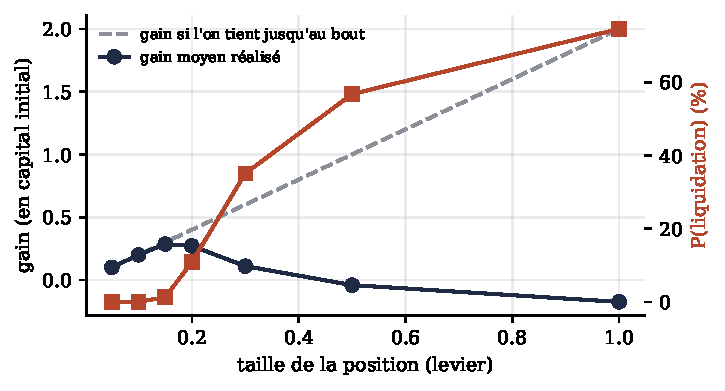
\includegraphics[width=0.6\textwidth]{ch17/spirale_marge.pdf}
\caption{Un arbitrage dont la convergence est certaine : le gain promis croît avec la taille, le gain réalisé passe par un maximum puis devient négatif, car la probabilité d'être liquidé avant la convergence explose.}
\label{c17:fig:margin}
\end{figure}

\paragraph{Lecture.} La convergence est garantie, et pourtant un arbitragiste trop levé perd de l'argent en moyenne. Le gain espéré est maximal pour une taille modeste ($L \approx 0{,}15$), bien en dessous de ce que suggère le \og gain certain\fg. La leçon s'applique directement aux stratégies de base et de \emph{funding} du chapitre~14 : la convergence à l'échéance ne protège pas d'une liquidation avant l'échéance. Le levier se choisit en fonction du \emph{pire élargissement plausible}, pas du gain attendu.

\subsection{La foule : août 2007}

\citet{khandanilo2011} analysent la semaine du 6 août 2007, pendant laquelle de nombreux fonds d'arbitrage statistique sur actions ont subi des pertes très inhabituelles, suivies d'un rebond partiel. Leur explication : beaucoup de fonds détenaient des portefeuilles semblables (mêmes facteurs, mêmes signaux) ; le débouclage rapide de l'un d'eux a fait bouger les prix contre tous les autres, ce qui a déclenché d'autres débouclages. Une stratégie est d'autant plus exposée qu'elle est populaire : le \emph{pairs trading} sur grandes capitalisations est l'une des stratégies quantitatives les plus répandues.

% =====================================================================
\section{Ce que vaut la diversification}
% =====================================================================

\begin{proposition}\label{c17:prop:div}
Soit un portefeuille équipondéré de $N$ paires, chacune de volatilité $\sigma$, avec une corrélation commune $\rho$ entre deux paires quelconques. Sa volatilité vaut
\[
\sigma_P = \sigma\sqrt{\frac1N + \rho\Big(1 - \frac1N\Big)}, \qquad\text{et}\qquad N_{\text{eff}} = \frac{\sigma^2}{\sigma_P^2} = \frac{N}{1 + (N-1)\rho}.
\]
\end{proposition}
\begin{proof}
Avec des poids $1/N$, $\Var\big(\frac1N\sum_i r_i\big) = \frac1{N^2}\big(\sum_i\Var(r_i) + \sum_{i\ne j}\Cov(r_i,r_j)\big) = \frac{1}{N^2}\big(N\sigma^2 + N(N-1)\rho\sigma^2\big) = \sigma^2\big(\frac1N + \rho\frac{N-1}{N}\big)$. Le nombre effectif est le nombre de paires indépendantes qui donneraient la même volatilité : $\sigma^2/N_{\text{eff}} = \sigma_P^2$.
\end{proof}

\begin{codebox}[ — E4, 20 paires]
\textbf{Volatilité relative et nombre effectif de paires :} $\rho = 0$ : $0{,}224$ ($N_{\text{eff}} = 20$) ; $\rho = 0{,}05$ : $0{,}312$ ($10{,}3$) ; $\rho = 0{,}1$ : $0{,}381$ ($6{,}9$) ; $\rho = 0{,}3$ : $0{,}579$ ($3{,}0$) ; $\rho = 0{,}6$ : $0{,}787$ ($1{,}6$). \textbf{Crise :} 20 paires de Sharpe annuel $1{,}6$ chacune, corrélation $0{,}05$ en temps normal ; une crise de 10 jours fait monter la corrélation à $0{,}6$ et inverse le rendement. Sur 10 ans, le drawdown maximal médian passe de $9{,}2$ à $34{,}1$ écarts-types quotidiens du portefeuille.
\end{codebox}

\paragraph{Lecture.} Une corrélation de seulement $0{,}05$ entre paires divise par deux le bénéfice de la diversification. Et la corrélation n'est pas stable : elle monte précisément pendant les crises, quand tous les arbitragistes liquident ensemble. Un portefeuille de 20 paires calibré sur la volatilité de temps normal subit en crise un drawdown près de quatre fois plus grand que prévu. Il faut donc dimensionner sur la volatilité \emph{de crise}, et diversifier entre familles de stratégies (actions, base, \emph{funding}, différents horizons) plutôt qu'entre paires d'une même famille.

% =====================================================================
\section{Les risques non statistiques}
% =====================================================================

\begin{description}
\item[Plateforme et contrepartie.] Une plateforme peut tomber en panne, geler les retraits ou faire faillite. Pour l'arbitrage inter-plateformes, le capital immobilisé sur chaque plateforme est exposé à ce risque, qui ne figure dans aucun \emph{backtest}. Règle : ne laisser sur une plateforme que la marge nécessaire, et plafonner l'exposition par contrepartie.
\item[Courtier et règles d'exécution.] Les CFD sont des contrats avec votre courtier, qui peut modifier les écarts, les heures, la marge ou refuser certains styles de trading. Le moteur \texttt{atjte} prévoit des plages d'interdiction (\emph{blackouts}) et des contrôles de marge à cet effet \citep{atjte}.
\item[Vente à découvert.] Les titres vendus doivent être empruntés ; le coût d'emprunt peut monter brutalement et le prêteur peut rappeler les titres, forçant à racheter.
\item[Opérations sur titres.] Dividendes, divisions, fusions, offres publiques : chacune peut créer un faux signal ou une rupture réelle.
\item[Réglementation et fiscalité.] Restrictions de vente à découvert en période de crise, régime fiscal des CFD et des cryptoactifs, obligations déclaratives des comptes à l'étranger.
\item[\emph{Prop firms}.] Les règles des \emph{prop firms} interdisent en général l'arbitrage de latence, la couverture croisée entre comptes et l'exploitation de défauts de cotation \citep{nexusfi}. Une stratégie d'arbitrage inter-plateformes déployée sur un compte de \emph{prop firm} risque l'annulation des gains et la fermeture du compte. Ces stratégies relèvent du capital propre.
\item[Risque opérationnel.] Bogues, erreurs de saisie (un ratio mal tapé), double lancement d'un robot, clés compromises (chapitre~15).
\end{description}

% =====================================================================
\section{Un cadre de limites de risque}
% =====================================================================

Les limites suivantes sont indépendantes du signal ; elles doivent être codées dans le moteur et vérifiées avant chaque ordre.

\begin{center}\small
\begin{tabularx}{\textwidth}{>{\raggedright}p{4.2cm}>{\raggedright\arraybackslash}X}
\toprule
Limite & Rôle \\
\midrule
Taille maximale par paire & Aucune paire ne pèse plus de $x\,\%$ du risque total. \\
Exposition nette maximale & La somme des deltas reste proche de zéro (neutralité réelle au marché). \\
Exposition non couverte maximale & Au-delà, couverture forcée ou arrêt (chapitre~15). \\
Perte journalière maximale & Arrêt de toutes les nouvelles positions pour la journée. \\
Drawdown maximal & Réduction de moitié de la taille à $-D/2$, arrêt complet à $-D$, revue obligatoire. \\
Exposition par plateforme & Capital maximal immobilisé chez chaque contrepartie. \\
Stop par paire & $|z| > 4$ ou durée $> 3$ demi-vies. \\
Plages interdites & Annonces macroéconomiques, ouvertures, maintenances des plateformes. \\
\bottomrule
\end{tabularx}
\end{center}

% =====================================================================
\section{Ce que la théorie apporte, et ses limites}
% =====================================================================

\paragraph{Apports.} Un ordre de grandeur du levier raisonnable (une fraction de Kelly), une comparaison chiffrée des protections contre la rupture, une démonstration qu'un arbitrage certain peut ruiner, et une formule simple de la diversification réelle.

\paragraph{Limites.} Les expériences supposent des lois connues ; dans la réalité, $\mu$, $\sigma$, $\rho$ et la probabilité de crise sont inconnus et instables. Les épisodes qui comptent le plus (faillite d'une plateforme, crise de liquidité générale) sont rares et mal représentés dans les données. La gestion du risque consiste donc moins à optimiser qu'à survivre : petites tailles, limites dures, diversification entre familles de stratégies.

% =====================================================================
\section{Fiche à recopier au tableau blanc}
% =====================================================================

\begin{whiteboard}
\begin{itemize}[leftmargin=1.2em]
\item \textbf{Kelly :} $g(f) \approx f\mu - \tfrac12 f^2\sigma^2$ ; $f^\star = \mu/\sigma^2$ ; $g(f^\star) = SR^2/2$ ; $g(2f^\star) = 0$ ; en pratique $0{,}1$ à $0{,}25\,f^\star$.
\item \textbf{Ciblage de volatilité :} $w_t = \min(\sigma^\ast/\hat\sigma_t, L_{\max})$, $\hat\sigma_t$ estimée sur le passé.
\item \textbf{Protections :} stop $|z|>4$ (quasi gratuit) ; durée $> 3$ demi-vies ; CUSUM $S^\pm_t = \max(0, S^\pm_{t-1} \pm z_t - k)$, alarme si $> h$.
\item \textbf{Limites de l'arbitrage :} perte latente $\Rightarrow$ appel de marge $\Rightarrow$ liquidation au pire moment ; levier choisi sur le pire élargissement.
\item \textbf{Diversification :} $\sigma_P = \sigma\sqrt{1/N + \rho(1-1/N)}$ ; $N_{\text{eff}} = N/(1+(N-1)\rho)$ ; $\rho$ monte en crise.
\item \textbf{Hors statistique :} plateforme, contrepartie, courtier, emprunt de titres, opérations sur titres, réglementation, \emph{prop firms}, erreurs opérationnelles.
\end{itemize}
\end{whiteboard}

% =====================================================================
\section{Exercices}
% =====================================================================

\begin{exercise}
Une stratégie a un Sharpe annuel de $1{,}5$ et une volatilité de 4\,\% par an sans levier. Calculez $f^\star$, la volatilité correspondante et la croissance à $f^\star$ et à $f^\star/4$.
\end{exercise}

\begin{exercise}
Montrez que la croissance $g(f)$ est symétrique autour de $f^\star$, c'est-à-dire $g(f^\star - a) = g(f^\star + a)$. Pourquoi la figure~\ref{c17:fig:kelly} confirme-t-elle ce résultat ?
\end{exercise}

\begin{exercise}
Avec 30 paires corrélées à $\rho = 0{,}08$, quel est le nombre effectif de paires ? Combien faudrait-il de paires pour atteindre $N_{\text{eff}} = 10$ ? Est-ce possible ?
\end{exercise}

\begin{exercise}[à coder]
Dans E3, remplacez la règle de liquidation par une règle de réduction : à chaque fois que la perte atteint 40\,\% du capital, on divise la position par deux. Comparez le gain moyen et la probabilité de perdre plus de 75\,\%.
\end{exercise}

\begin{exercise}[à coder]
Calibrez $h$ du CUSUM ($k = 0{,}5$) pour obtenir 2\,\% de fausses alarmes sur 1\,000 jours dans le monde stable de E2. Quel délai de détection obtenez-vous ?
\end{exercise}

\begin{exercise}[données réelles]
Rédigez la fiche de limites de risque (section précédente) pour votre propre compte, avec des nombres. Quelle perte maximale acceptez-vous sur une journée, un mois, au total ? Déduisez-en la taille maximale de votre première paire.
\end{exercise}

% =====================================================================
\section{Pour aller plus loin}
% =====================================================================

\begin{toread}
\begin{itemize}[leftmargin=1.2em]
\item \citet{thorp2006} : sections sur le critère de Kelly en temps continu et sur l'usage de fractions de Kelly.
\item \citet{shleifer1997} : section II (modèle) et section IV (conséquences empiriques) ; lecture indispensable.
\item \citet{brunnermeier2009} : la spirale entre liquidité de marché et liquidité de financement.
\item \citet{khandanilo2011} : sections sur la simulation d'une stratégie de retour à la moyenne en août 2007.
\item \citet{page1954} : l'article original du CUSUM, court.
\item Chapitre~14 de ce cours, pour relire les stratégies de base à la lumière de la spirale de marge.
\end{itemize}
\end{toread}

\section{Scripts du chapitre}
\sloppy\noindent\texttt{code/ch17/ch17\_risk.py} : E1 (figure~\ref{c17:fig:kelly}), E2 (figure~\ref{c17:fig:protect}), E3 (figure~\ref{c17:fig:margin}), E4. Module : \texttt{src/arbhub/risk/sizing.py} ; tests : \texttt{tests/test\_risk.py}.
